% !TEX TS-program = pdflatex
% !TEX encoding = UTF-8 Unicode

% This is a simple template for a LaTeX document using the "article" class.
% See "book", "report", "letter" for other types of document.

\documentclass[20pt]{article} % use larger type; default would be 10pt

\usepackage[utf8]{inputenc} % set input encoding (not needed with XeLaTeX)

%%% Examples of Article customizations
% These packages are optional, depending whether you want the features they provide.
% See the LaTeX Companion or other references for full information.

%%% PAGE DIMENSIONS
\usepackage{geometry} % to change the page dimensions
\geometry{a4paper} % or letterpaper (US) or a5paper or....
% \geometry{margin=2in} % for example, change the margins to 2 inches all round
% \geometry{landscape} % set up the page for landscape
%   read geometry.pdf for detailed page layout information

\usepackage{graphicx} % support the \includegraphics command and options

% \usepackage[parfill]{parskip} % Activate to begin paragraphs with an empty line rather than an indent

%%% PACKAGES
\usepackage{booktabs} % for much better looking tables
\usepackage{array} % for better arrays (eg matrices) in maths
\usepackage{paralist} % very flexible & customisable lists (eg. enumerate/itemize, etc.)
\usepackage{verbatim} % adds environment for commenting out blocks of text & for better verbatim
%\usepackage{subfig} % make it possible to include more than one captioned figure/table in a single float
\usepackage{mathtools}
\usepackage{graphicx} % supports images in latex
% These packages are all incorporated in the memoir class to one degree or another...

\usepackage{url}
\usepackage{graphicx}
\usepackage{subcaption}

%%% Other stuff
\DeclarePairedDelimiter\ceil{\lceil}{\rceil}
\DeclarePairedDelimiter\floor{\lfloor}{\rfloor}

%%% HEADERS & FOOTERS
\usepackage{fancyhdr} % This should be set AFTER setting up the page geometry
\pagestyle{fancy} % options: empty , plain , fancy
\renewcommand{\headrulewidth}{0pt} % customise the layout...
\lhead{}\chead{}\rhead{}
\lfoot{}\cfoot{\thepage}\rfoot{}

%%% SECTION TITLE APPEARANCE
\usepackage{sectsty}
\allsectionsfont{\sffamily\mdseries\upshape} % (See the fntguide.pdf for font help)
% (This matches ConTeXt defaults)

%%% ToC (table of contents) APPEARANCE
\usepackage[nottoc,notlof,notlot]{tocbibind} % Put the bibliography in the ToC
\usepackage[titles,subfigure]{tocloft} % Alter the style of the Table of Contents
\renewcommand{\cftsecfont}{\rmfamily\mdseries\upshape}
\renewcommand{\cftsecpagefont}{\rmfamily\mdseries\upshape} % No bold!

%%% graphics path
\usepackage{amsmath}
\usepackage{listings}
%\begin{lstlisting}[language=java]
%\end{lstlisting}



%%% END Article customizations

%%% nice things to keep around
%\begin{figure}[!htbp]
%  	\centering
%   	\begin{subfigure}[p]{0.5\linewidth}
%    	\includegraphics[width=\linewidth]{}
%   	\end{subfigure}
%\end{figure} 

% \noindent\rule{2cm}{0.4pt} 
%%% puts a small horizontal line

% \mathcal{O} 
%%% big O notation

% \begin{table}[!htbp]
% \caption{Forward slash.}
% \[\begin{array}{c|ccccc} 
% abc/def & 1 & 2 & 3 & 4 & 5\\
% \hline
% 1 & a & b & c & d & e\\
% 2 & f & g & h & i & j\\
% 3 & k & l & m & n & o\\
% \end{array}\]
% \end{table}

%%% The "real" document content comes below...

\title{Computational Statistics Final Report}
\author{Liam Dillingham, Jose Azucena, Kagan Dupuy-Reagan}
%\date{} % Activate to display a given date or no date (if empty),
         % otherwise the current date is printed 

\begin{document}
\maketitle

\section{Introduction}
The data which I wanted to analyze is the NCI60 cell data, a dataset which contains 64 samples of varieties of cancer, with 6830 features per observation.  Within this dataset, there exists 14 different types of cancer.  While this is supposed to  be an unsupervised learning project, I experimented with the data, using the provided labels to hone my intuition about how to improve my model, and to study the learning process.

\section{Preprocessing}
The first thing I did was utilize R's \textbf{prcomp()} method, which utilizes the more numerically accurate \textit{singular value decomposition} algorithm for computing \textit{Principal Component Analysis}.  I of course standardized the data using the arguments to the function to scale and center the data.  I then exported the \textit{PCA} transformed data as well as the labels into separate \textit{*.csv} files to be used in python.  Some analytical operations are easier in \textit{R}, while others are easier in \textit{python}, which is why I made these decisions (It's mostly personal preference).

\section{First Analysis}
Although we are given the labels for the data here, this is supposed to be an unsupervised learning project, so initially I produced results in absence of the labels.  The first action to perform after the initial principal componenet analysis is a sufficient number of PC's such that I can obtain at least 85\% of the total variance.  I selected 39, which gave me slightly more than 85\%, in fact, we can actually observe the threshold with the small table I produced below:
\begin{itemize}
\item 37 PC's $\rightarrow$ 84.9\%
\item 38 PC's $\rightarrow$ 85.8\%
\item 39 PC's $\rightarrow$ 86.6\%
\end{itemize}
\newpage
This selection was to bump me slightly over the 85\% threshold.  I then wanted to cluster this data using KMeans.  which $k$ to select isn't immediately obvious, so I used an algorithm which computes the clusters for many different values of $k$, and plots the inertia of the groups.  We can see the result of this below: 
\begin{figure}[!htbp]
  	\centering
   	\begin{subfigure}[p]{0.7\linewidth}
    	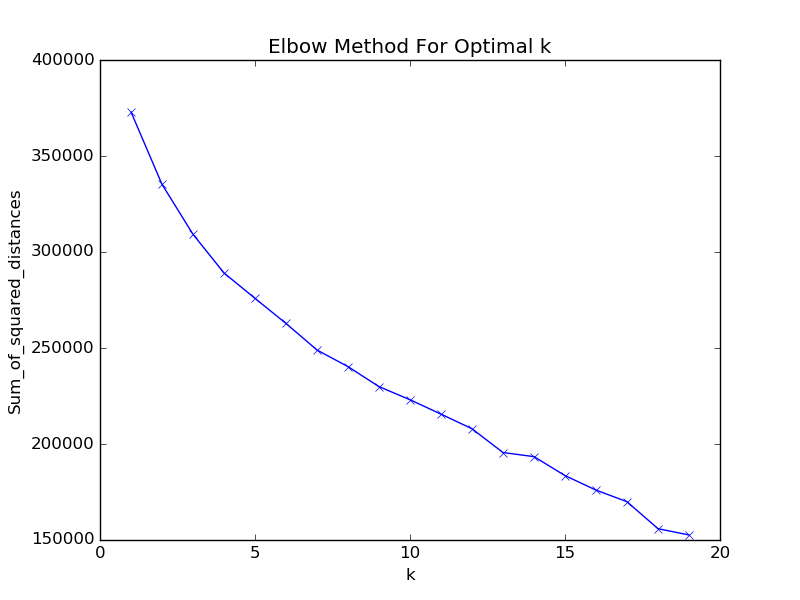
\includegraphics[width=\linewidth]{./figures/kmax20.png}
   	\end{subfigure}
\end{figure}

There are a few good selections of $k$ for this graph, but the smallest $k$ which reduces the inertia appears to be $k=4$.  So I selected it, and ran the algorithm again.  The results are fairly high-dimensional, so I need a way to visualize the results.  This is where the projection algorithm, \textit{t-distributed stochastic neighbor embedding (TSNE)} comes in. This algorithm measures the distance between a given point $p$ and all other points, say $q$. It then maps these distances to a t-distribution, where $p$ is at the center of the distribution.  Points far away from $p$ are in the far tails of the distribution, while points nearby are close to the center.  It then builds a similarity matrix of these distances/probabilites.  Then, it projects randomly the points to the desired dimension, and uses gradient descent to nudge the points in the new space to a proper distance to $p$. It does this for all points.  The downside is that while it preserves the local structure of points to their neighbors, it destroys the global structure of the data.  There are a few hyperparameters that go with this algorithm which we can examine in detail.

\newpage
\textit{Perplexity} is a value which tries to balance the attention between local and global aspects of the data.  It is typically advised to select a value smaller than the number of points  ($n=64$). \textit{(Wattenberg, 2016)}.  By selecting a lower perplexity, we are very focued on the local structure of the data, and group points by only their closest neighbors.  By selecting larger values, the whole dataset begins to become a single neighborhood:
\begin{figure}[!htbp]
  	\centering
   	\begin{subfigure}[p]{0.45\linewidth}
    	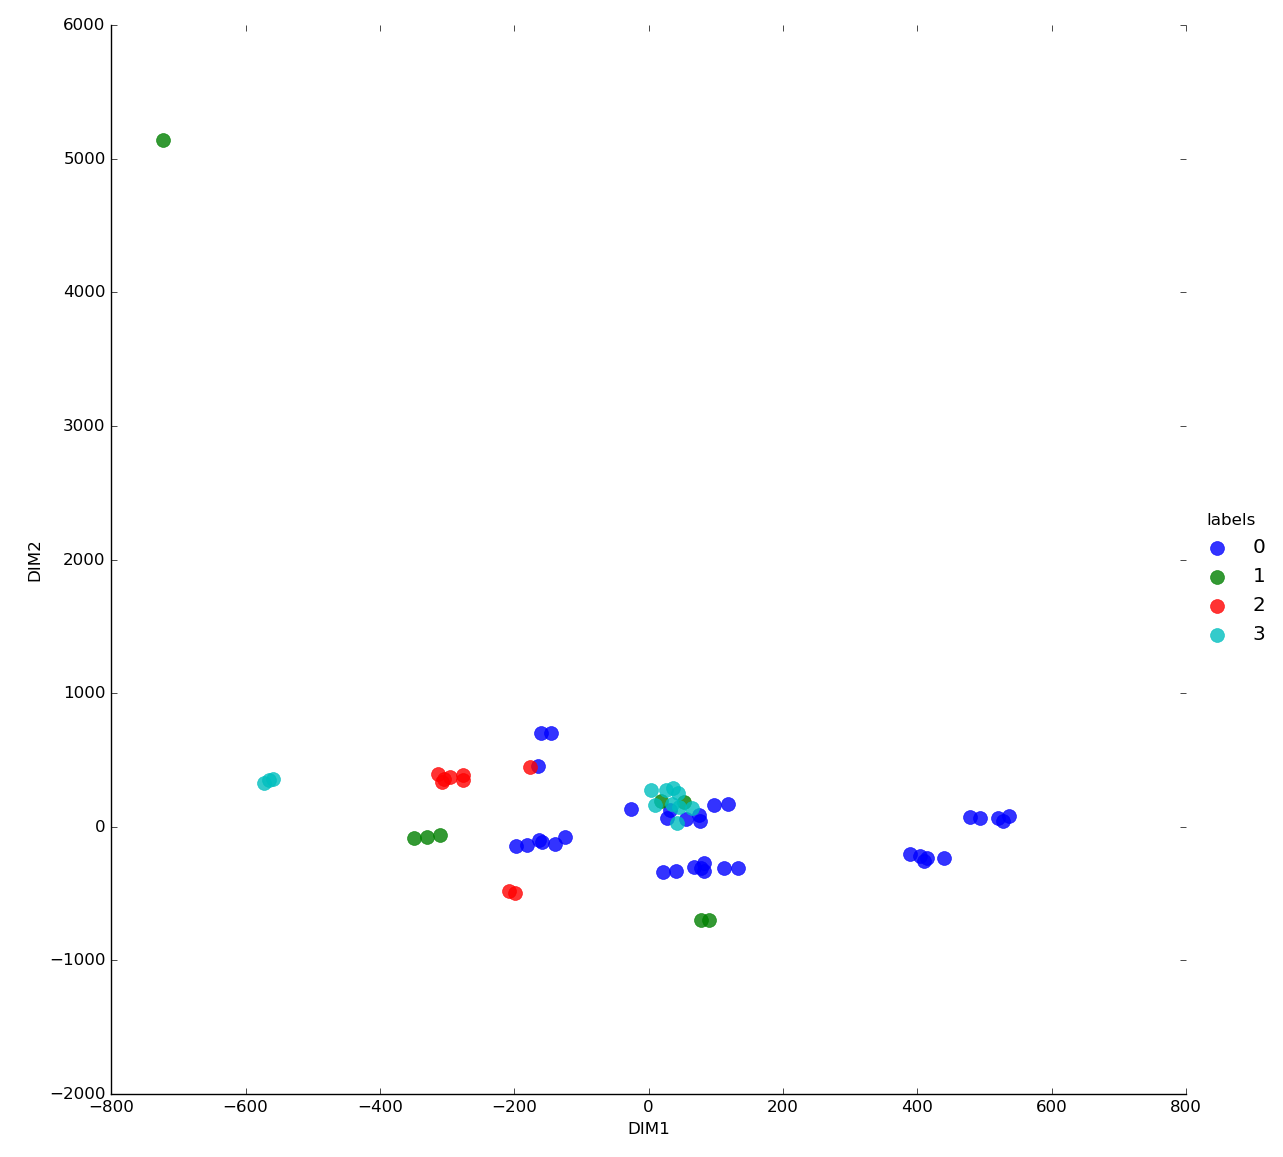
\includegraphics[width=\linewidth]{./figures/lowp.png}
	\caption{perplexity = 1}
   	\end{subfigure}
  	\centering
   	\begin{subfigure}[p]{0.45\linewidth}
    	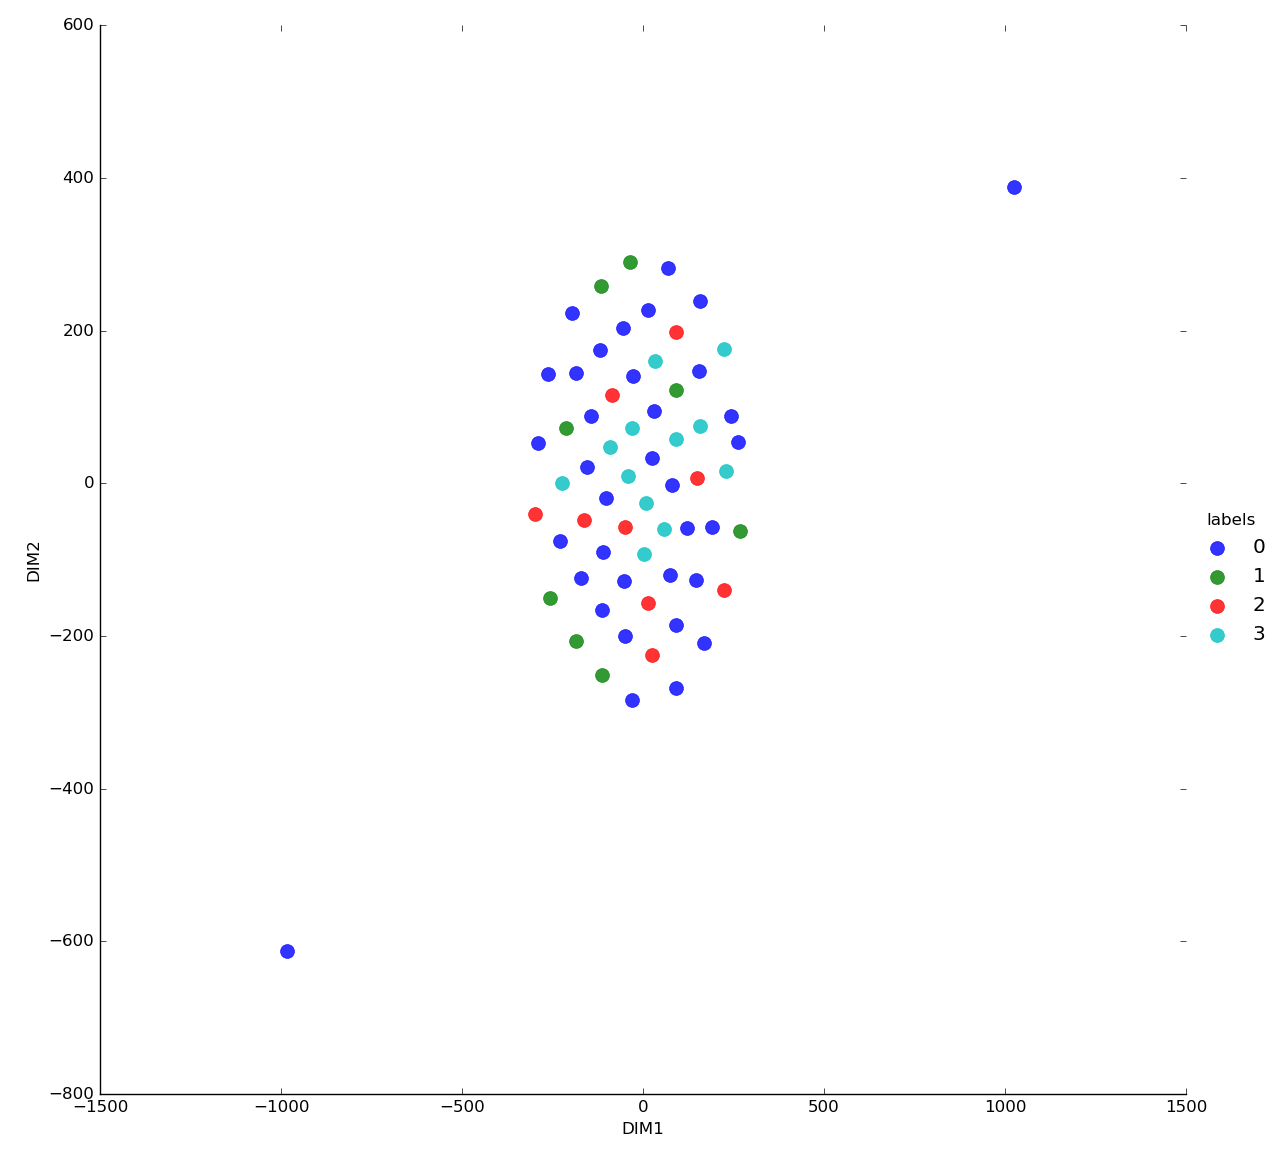
\includegraphics[width=\linewidth]{./figures/highp.png}
	\caption{perplexity = 100}
   	\end{subfigure}
\end{figure}

There is another important hyper-parameter called \textit{early exaggeration}.  This functions to strengthen the ties between local points to create smaller clusters during initial optimization \textit{(keitakurita, 2018)}
\begin{figure}[!htbp]
  	\centering
   	\begin{subfigure}[p]{0.45\linewidth}
    	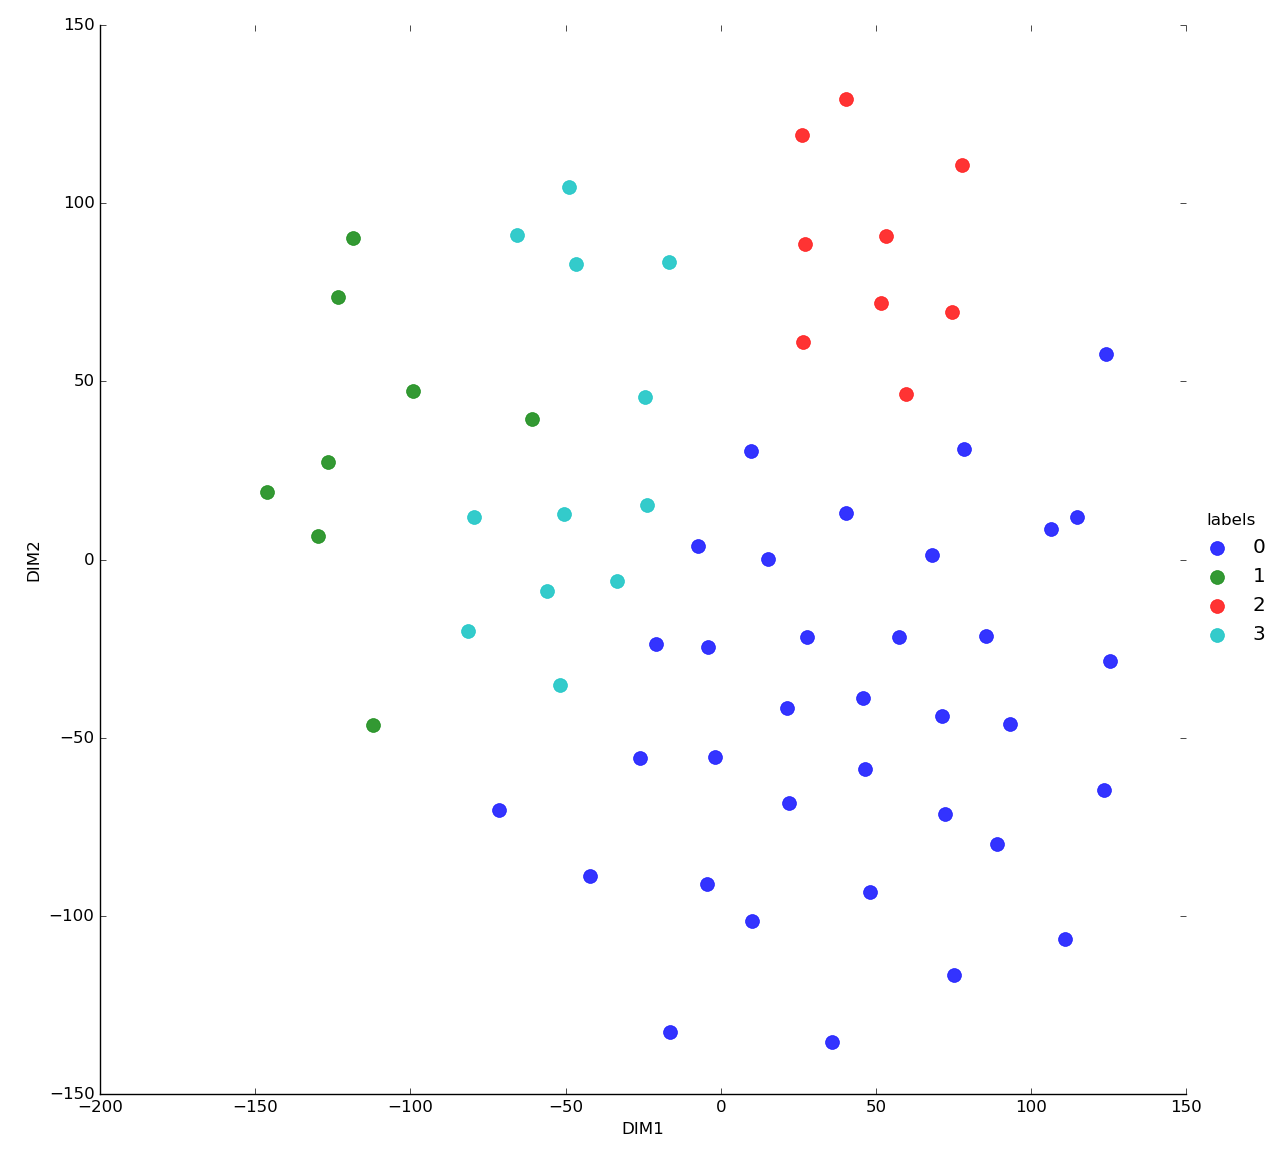
\includegraphics[width=\linewidth]{./figures/eelow.png}
	\caption{early exaggeration = 1}
   	\end{subfigure}
  	\centering
   	\begin{subfigure}[p]{0.45\linewidth}
    	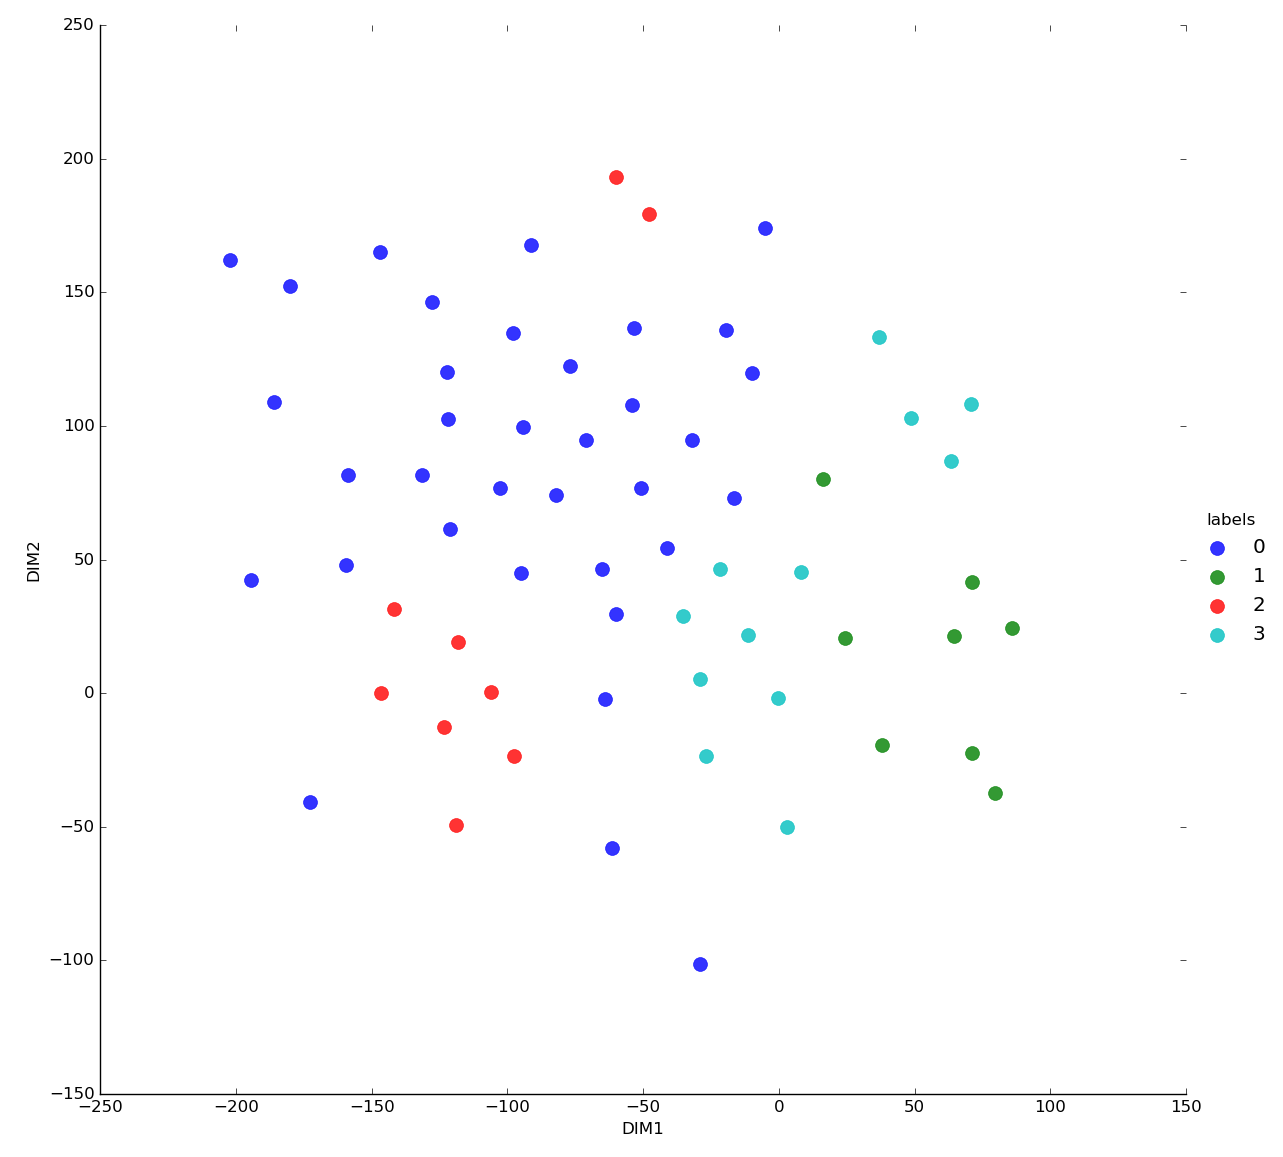
\includegraphics[width=\linewidth]{./figures/eehigh.png}
	\caption{early exaggeration = 100}
   	\end{subfigure}
\end{figure}
As we can see, it doesn't seem to affect the output of the algorithm much, other than the red cluster is now split in two.  What can cause this is that during the optimization, some of the red points were closer to some of the other blue points, and the early exaggeration caused them to converge together too early before they could be optimized closer to their real red neighbors.  So early exaggeration has the potential to create \textit{false clusters}. \textit{(keitakurita, 2018)}
\newpage

There are other hyperparameters, such as the \textit{intial seed}, the number of \textit{iterations}, the \textit{learning rate}, the \textit{tolerance} for convergence, and so on.  These hyperparamters are not exclusive to \textit{t-SNE}, so I didn't find interest in describing them in depth. By playing with these hyperparameters, we can maximize the profoundness of the visualization, and using our intuition, we can visually verify the results of our KMeans clusters.  This is the result of some hand selected hyperparamters for KMeans $k=4$.
\begin{figure}[!htbp]
  	\centering
   	\begin{subfigure}[p]{0.7\linewidth}
    	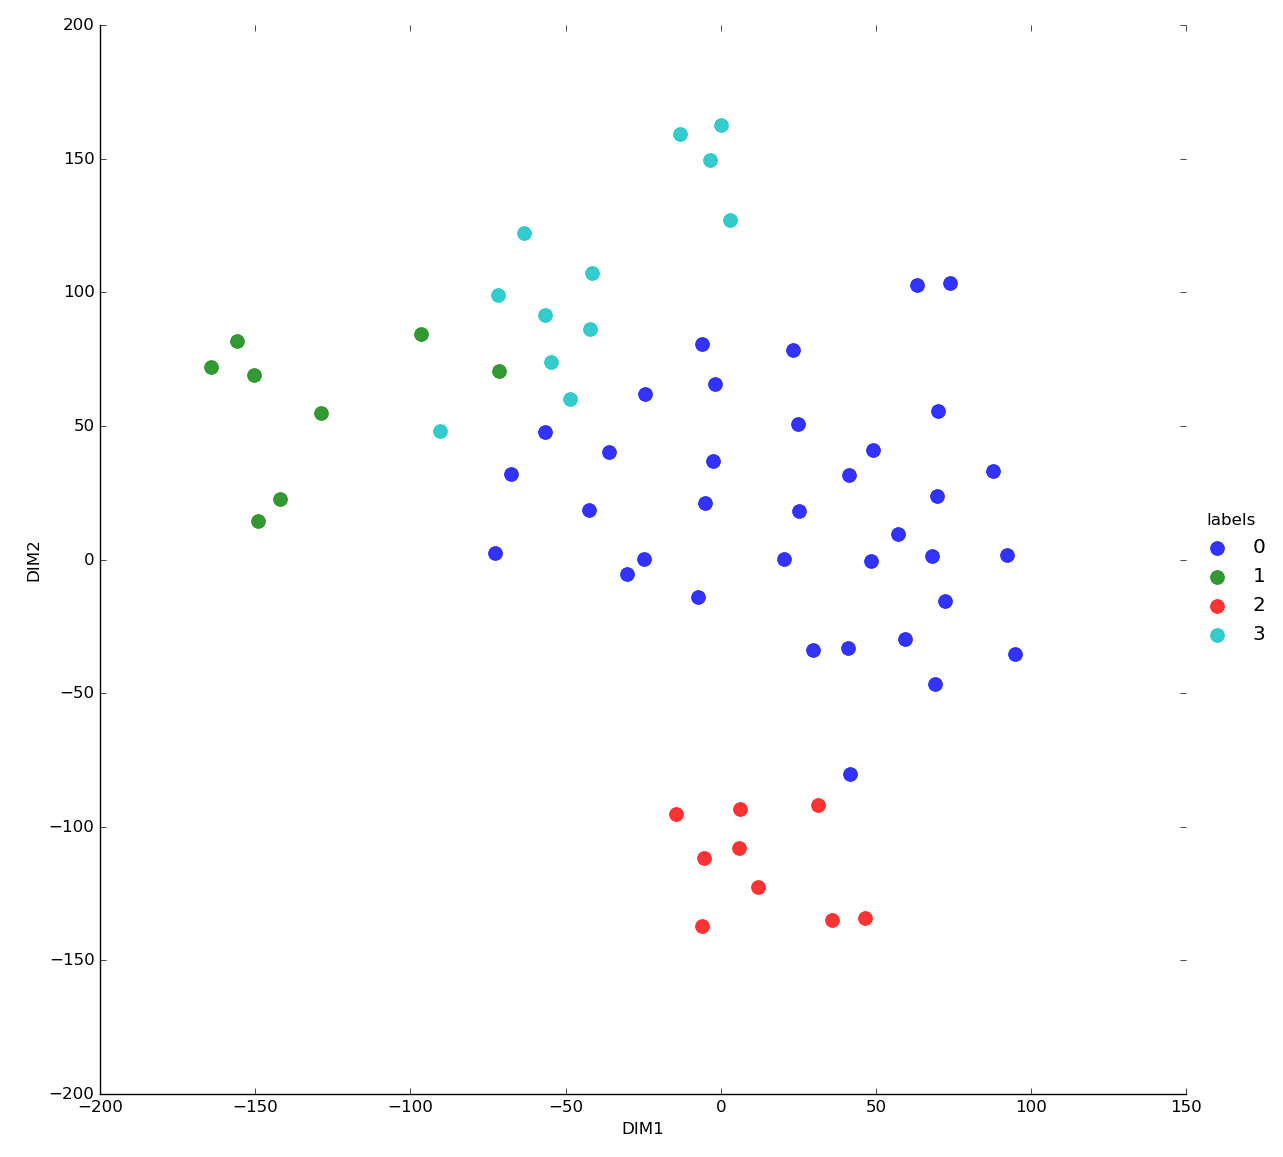
\includegraphics[width=\linewidth]{./figures/plot4.png}
   	\end{subfigure}
\end{figure}
These clusters look well, however, if we observe the plot, the green, light blue, and dark blue clusters are very close.  This could cause some misclassifications if we don't know the actualy number of groups in the data (It's actually 14 groups).  In addition, while the red cluster is very well separated from the group, there is a blue point close to it, which may be the result of a misclassified blue point.  If we go back to our chart, we can see another elbow at $k = 7$, as well as a very significant elbow at $k = 14$.  Lets try that one.
\newpage
\begin{figure}[!htbp]
  	\centering
   	\begin{subfigure}[p]{0.7\linewidth}
    	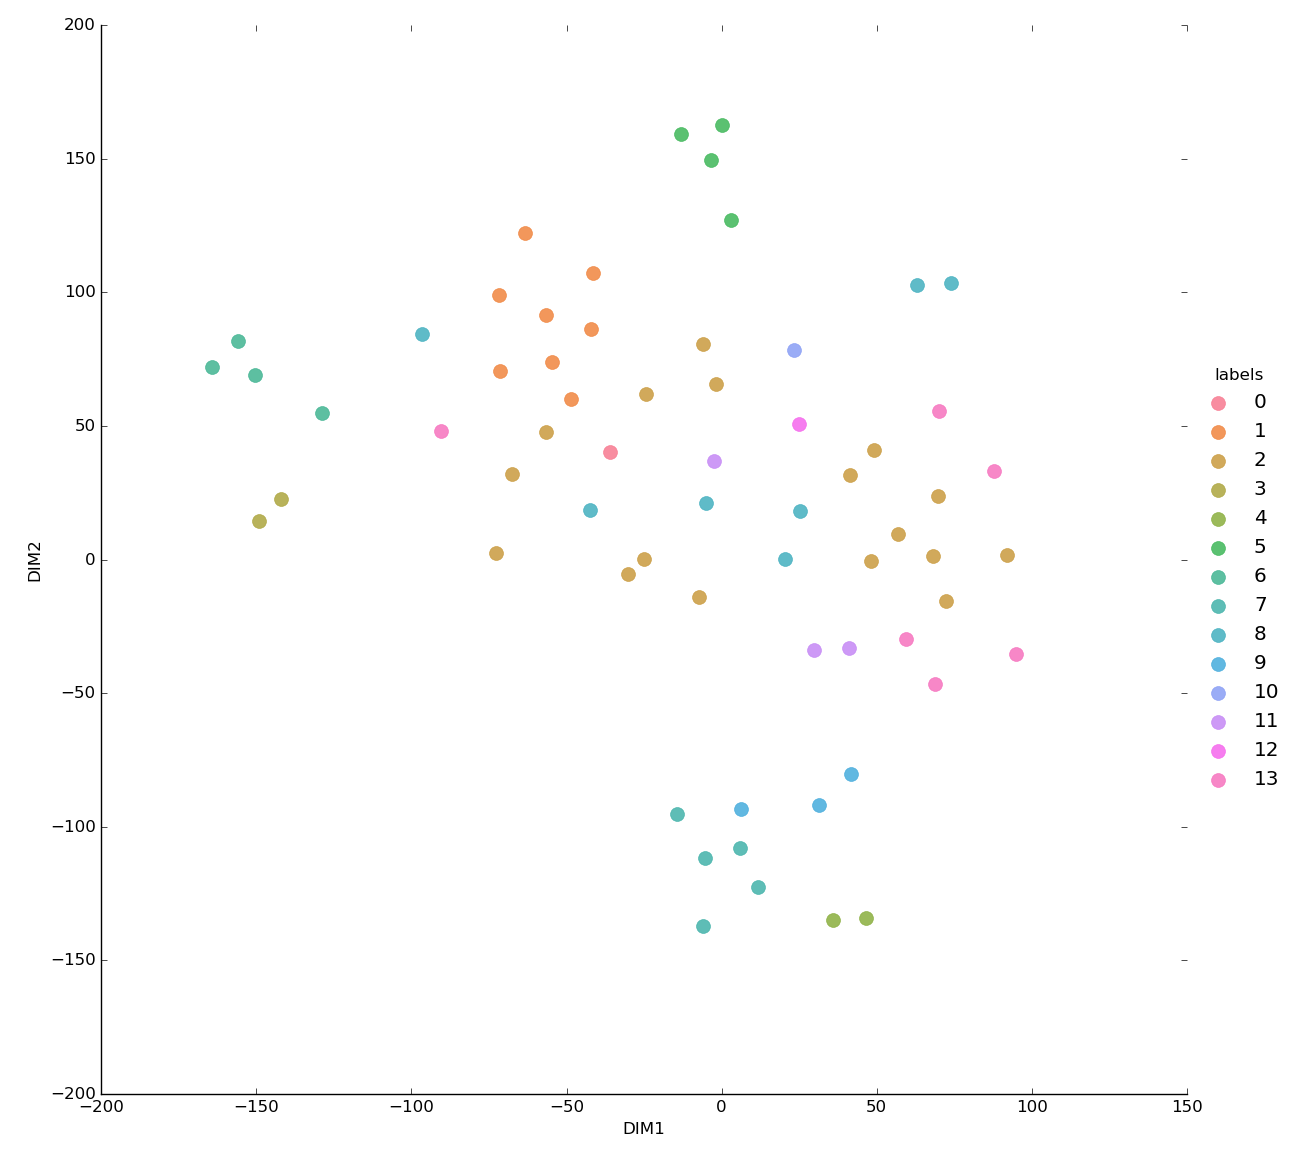
\includegraphics[width=\linewidth]{./figures/plot5.png}
   	\end{subfigure}
\end{figure}
Our plot now seems to be destroyed by the results of the new clustering.  This could be due to KMeans, or due to the way t-SNE performed.  Let's toy with the hyperparamters again and see if we can produce anything better.

I actually took this one step further.  Instead of doing random testing and waiting for the results, I instead produced an experiment similar to the optimal $k$ problem.  So after projecting the data down, I measured the squared distance between each point of the same cluster label, and summed it together. I did this for the perplexity values first, between 1 and 40, skipping every 2 values:
\begin{figure}[!htbp]
  	\centering
   	\begin{subfigure}[p]{0.6\linewidth}
    	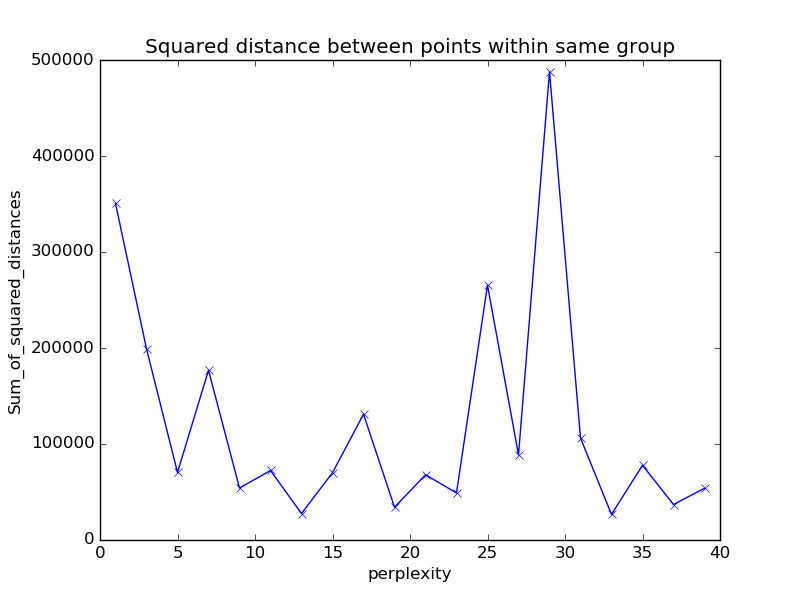
\includegraphics[width=\linewidth]{./figures/optimal_perp.png}
   	\end{subfigure}
\end{figure}

\newpage
This comes with the caveats that the hyperparamters are not independent of one another.  That is, if we were to test another hyperparamter with the same experiment, we need to fix all others.  Unfortunately, this can drastically change the results. For example, for the previous test of perplexity, the value of the early exaggeration was fixed at 10.  Let's run the test again with early exaggeration at 20, and see what the results look like:
\begin{figure}[!htbp]
  	\centering
   	\begin{subfigure}[p]{0.6\linewidth}
    	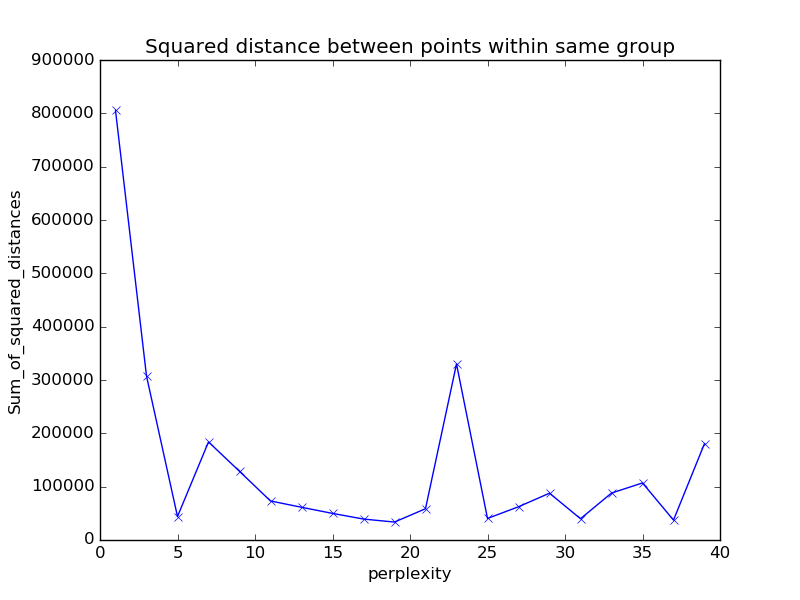
\includegraphics[width=\linewidth]{./figures/optimal_perp1.png}
   	\end{subfigure}
\end{figure}
My best guess is for some perplexity value we want to test, we run t-SNE with a large range of early exaggeration values, and sum them all together for that given perplexity value.  Whichever value of perplexity is the lowest (or we can compute the average distance instead of total distance) is the best perplexity value. This has the potential to take a very long time to compute, because of the complexity of the t-SNE algorithm, but I ran the algorithm again where for each perplexity value $p$, I tested 20 different early exaggeration values between 1 and 40, for 1000 iterations each.
\begin{figure}[!htbp]
  	\centering
   	\begin{subfigure}[p]{0.6\linewidth}
    	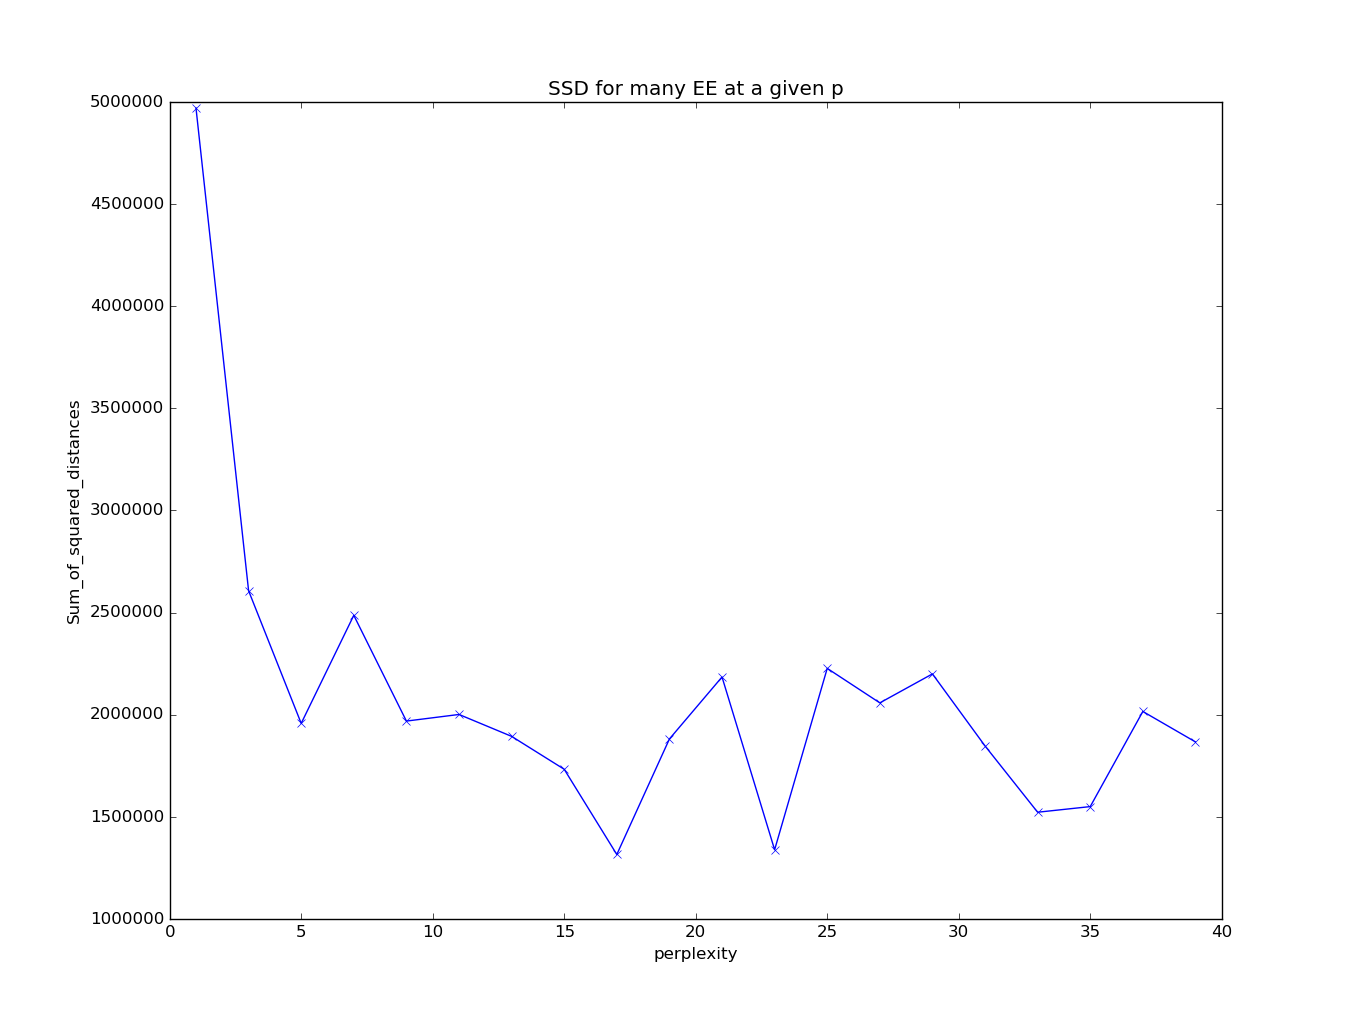
\includegraphics[width=\linewidth]{./figures/best_perp.png}
   	\end{subfigure}
\end{figure}
It seems as though the best value is about 17.  Now, we can flip the experiment around, and test early exaggeration values, or test random seeds, and so on.  But for now, lets pick a random value of early exaggeration, say 20 (that's about the middle of our testing) and a perplexity value of 17.
\begin{figure}[!htbp]
  	\centering
   	\begin{subfigure}[p]{0.7\linewidth}
    	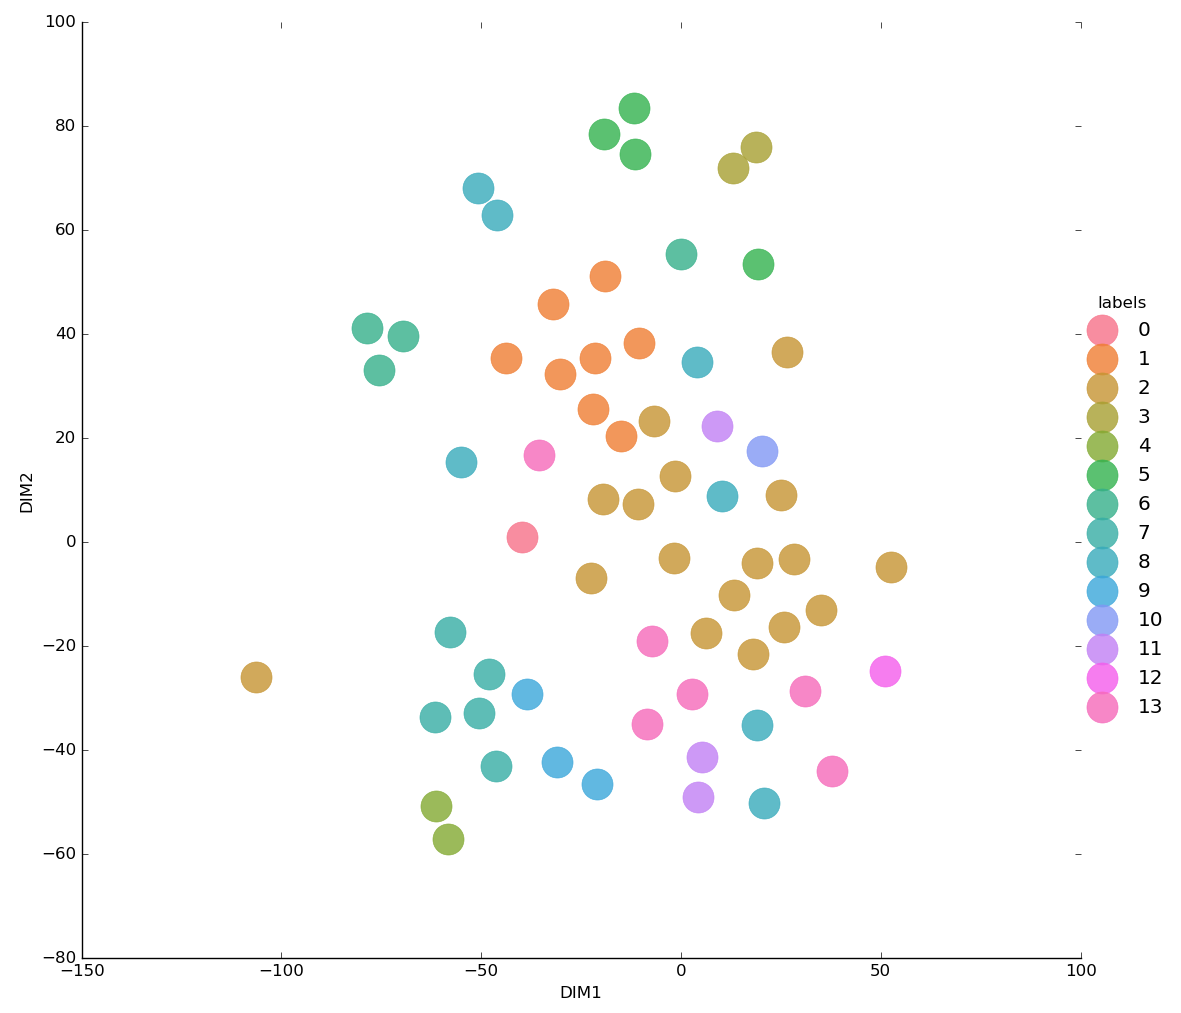
\includegraphics[width=\linewidth]{./figures/best_tsne.png}
   	\end{subfigure}
\end{figure}
Since the differences between the colors are so subtle, I scaled up the size of the points drastically to aid in the visualization.  We can see here that the groupings are much better, but how do we know that these are good classifications?  Let's run KMeans with many different fixed random seeds, and select the best one. Since KMeans can be made deterministic, if we can derive good results, they will be easily interpretable and reproducible.  

Another alternative is that KMeans may simply be the wrong clustering algorithm for the data.  It is however, quite popular, due to its deterministic behavior, after the centroid seeds have been randomly selected.  However, we can even control that.  By controlling the starting seed, we can actually compute the optimal starting seed for which to begin the centroids at.  For our selected value $k$, we want to run KMeans for several different seeds (perhaps 50) and observe the one which minimizes inertia.  If those results are still unsatisfactory, then we may move on and try other algorithms.  
\begin{figure}[!htbp]
  	\centering
   	\begin{subfigure}[p]{0.95\linewidth}
    	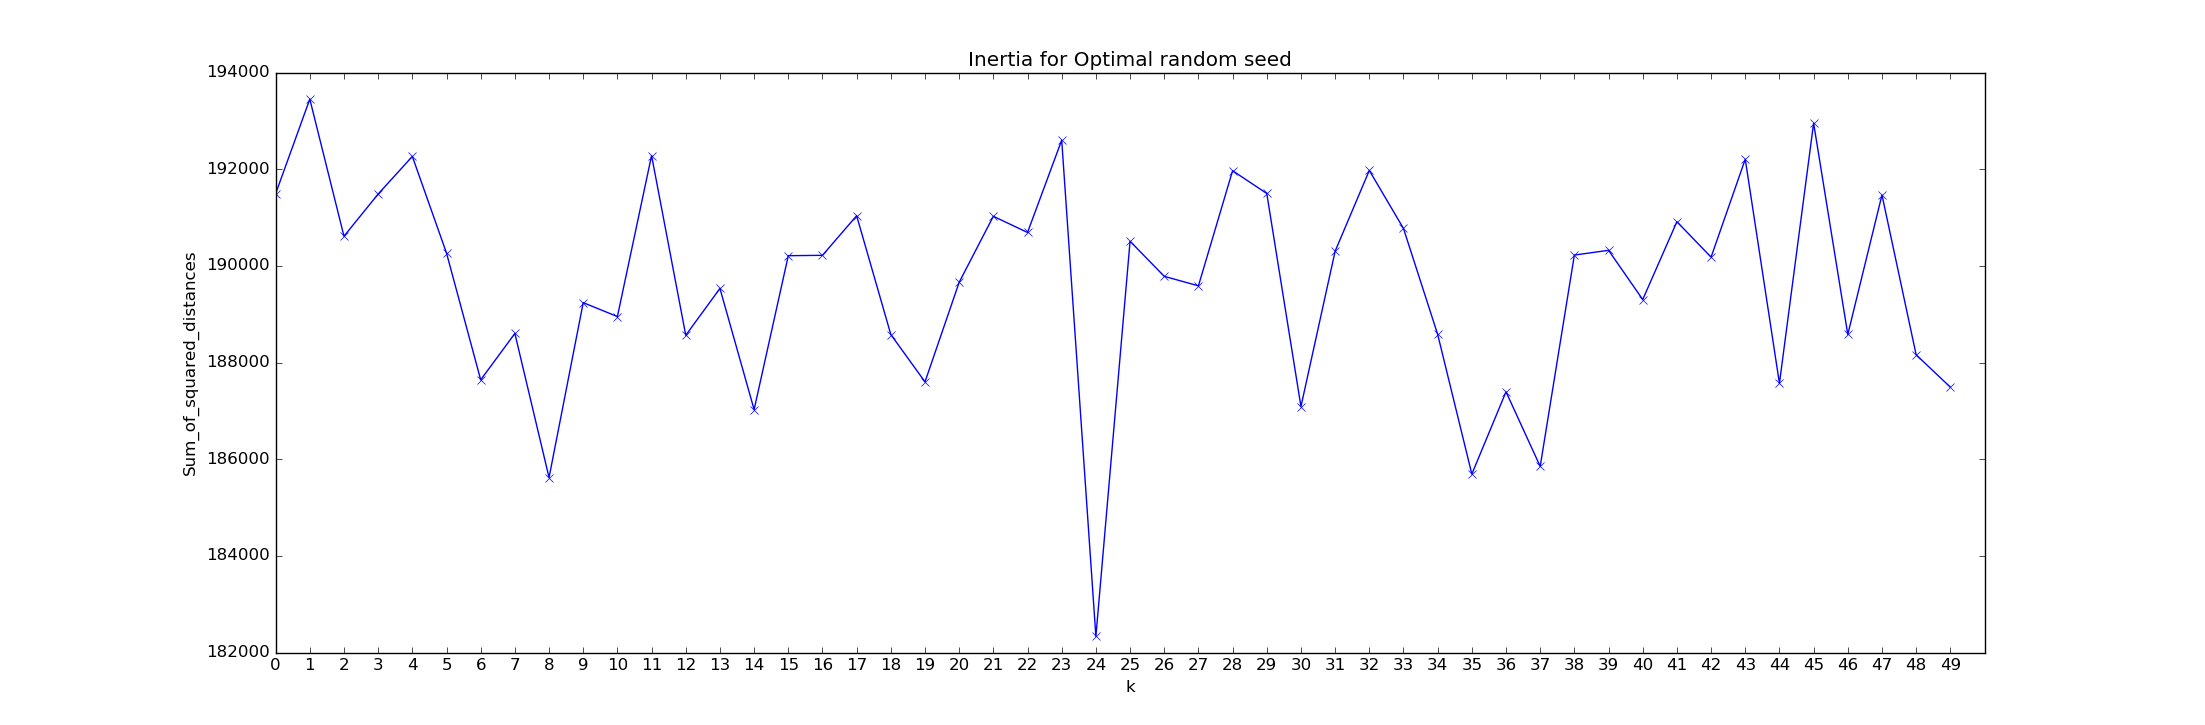
\includegraphics[width=\linewidth]{./figures/best_newseed.png}
   	\end{subfigure}
\end{figure}

\newpage
It may be difficult to read from the graph, but that seed value in which the inertia is very low is 24.  Lets re-run everything again with 24 as the seed and take a look at the graph. Also, because we have changed out clustering algorithm, we need to re-run the t-SNE optimization experiment, and re-derive our optimal perplexity value.
\begin{figure}[!htbp]
  	\centering
   	\begin{subfigure}[p]{0.5\linewidth}
    	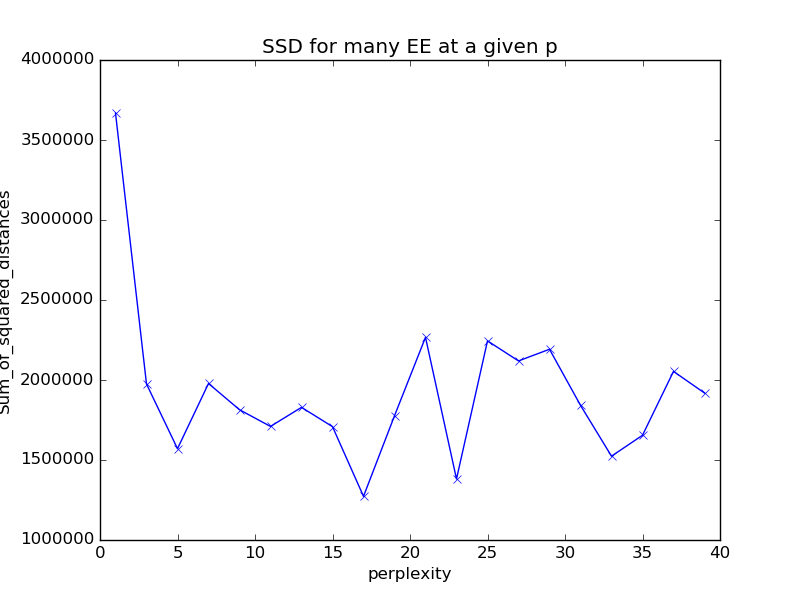
\includegraphics[width=\linewidth]{./figures/best_perp1.png}
   	\end{subfigure}
\end{figure}
This result is actually very interesting.  17 is still the best perplexity value, which goes to show that there is some consistency about the natural structure of the data. Below is the output of our new optimal clustering:
\begin{figure}[!htbp]
  	\centering
   	\begin{subfigure}[p]{0.7\linewidth}
    	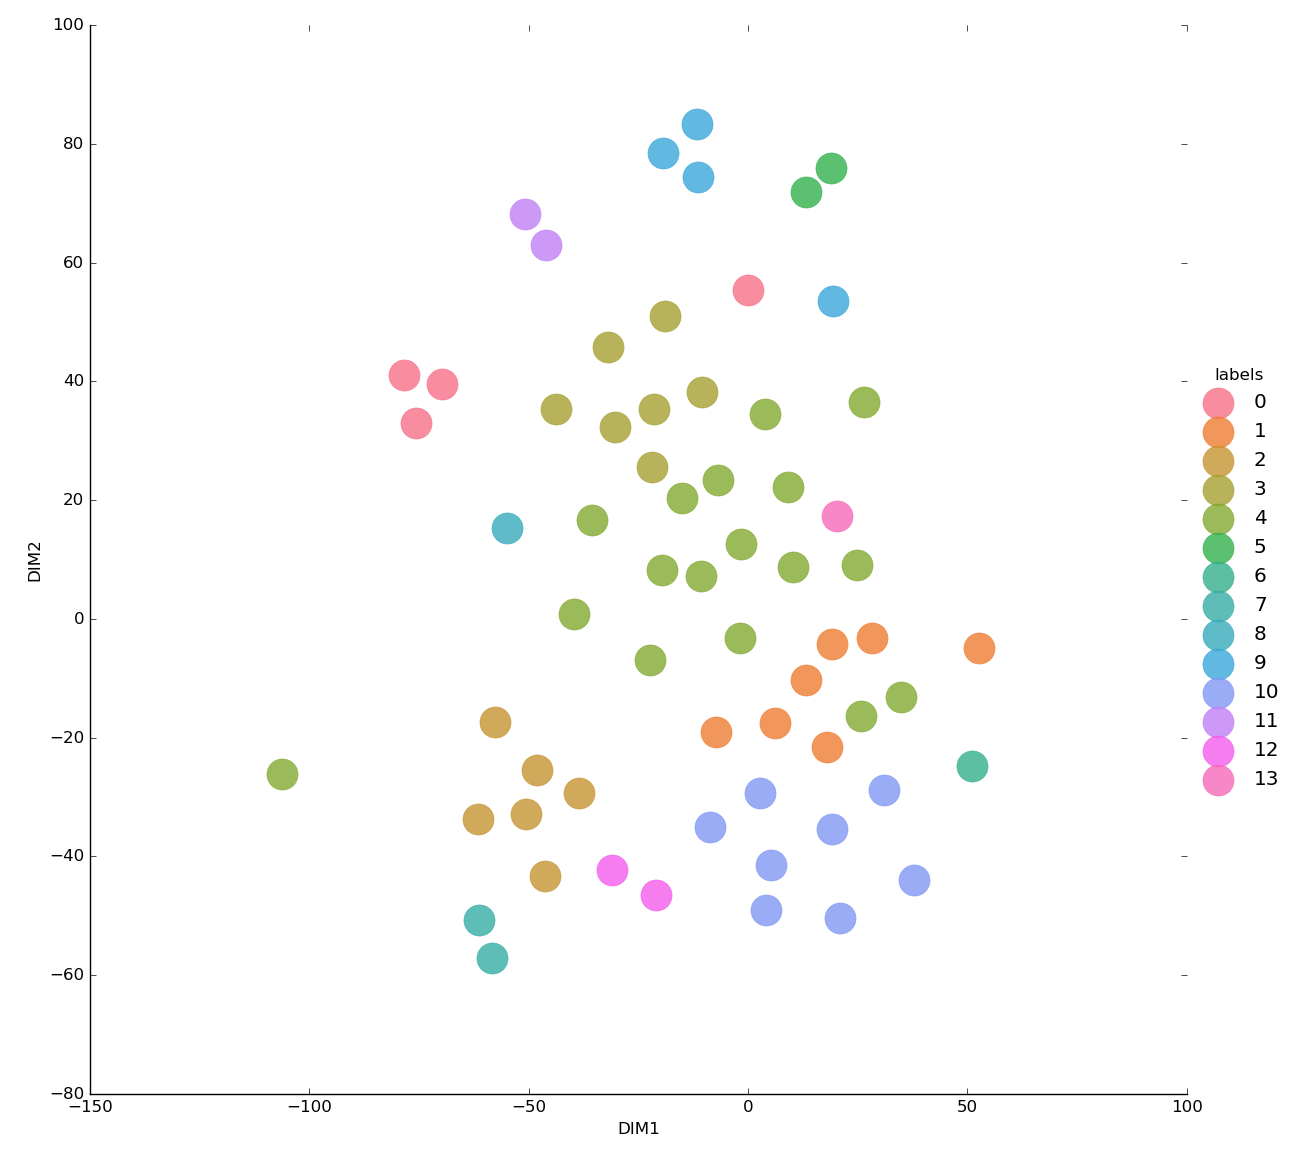
\includegraphics[width=\linewidth]{./figures/best_seed_tsne.png}
   	\end{subfigure}
\end{figure}

\newpage
If we import the labels and apply it to this graph, we can see how well the clustering works:
\begin{figure}[!htbp]
  	\centering
   	\begin{subfigure}[p]{1.2\linewidth}
    	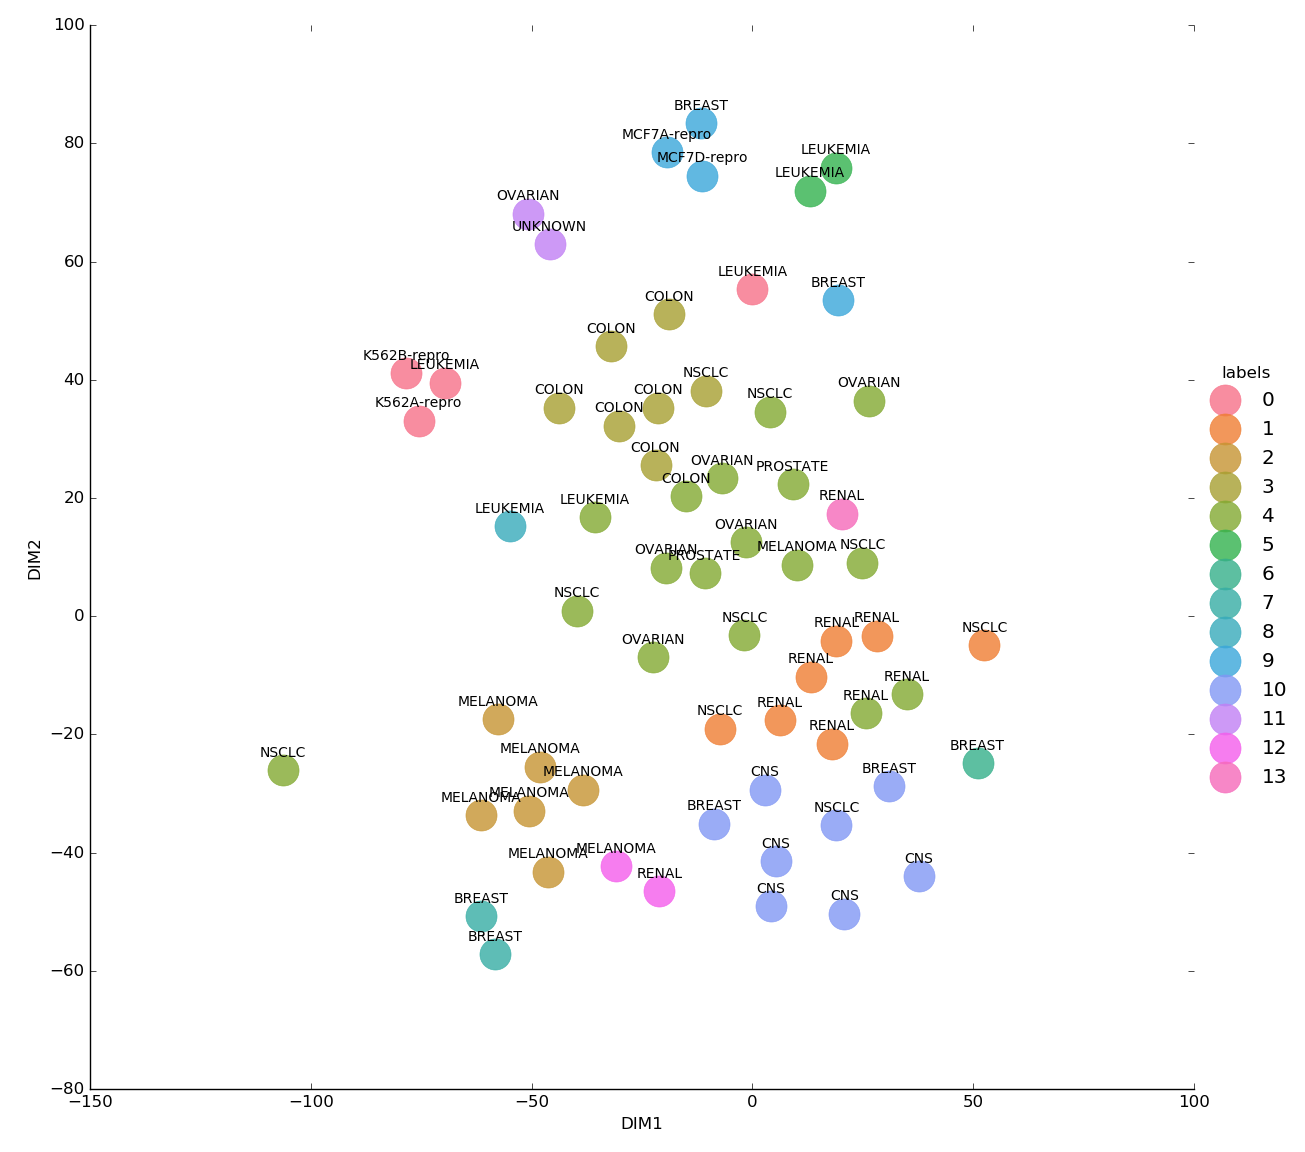
\includegraphics[width=\linewidth]{./figures/Best_clustering_labels.png}
   	\end{subfigure}
\end{figure}
I actually developed an algorithm to try and compute the misclassification rate of this data.  For each cluster, the algorithm computes the mode.  Then, for each label in the cluster that is not equal to the mode, it counts it as a misclassification.  It is worth noting that a group of size 1 cannot have an error greater than 0. And if there exists two modes for a group, then the "correct" one is picked at random.  For this experiment, we had 24 misclassifications using our accuracy method, which gives us an accuracy of about 62.5\% for correctly clustering the data groups apart.  Keep in mind that if we have two separate groups that all contain the same labels, that is still correct, as the groups are homogeneous from the other classes.

\newpage
 \begin{table}[!htbp]
 \caption{Misclassifications}
 \[\begin{array}{c|cccccccccccccc} 
 Error/Group & 0 & 1 & 2 & 3 & 4 & 5 &6&7&8&9&10&11&12&13\\
 \hline
 MissClass & 0 & 2 & 0 & 1 & 12 & 0 & 0 & 0 & 0 & 2 & 3 & 1 & 1 & 0\\
 \end{array}\]
 \end{table}

And we can see the actual groupings for the clustering below:
\begin{verbatim}
0  | ['K562B-repro', 'K562A-repro', 'LEUKEMIA', 'LEUKEMIA']
1  | ['NSCLC', 'RENAL', 'RENAL', 'RENAL', 'RENAL', 'RENAL', 'NSCLC']
2  | ['MELANOMA', 'MELANOMA', 'MELANOMA', 'MELANOMA', 'MELANOMA', 'MELANOMA']
3  | ['COLON', 'COLON', 'COLON', 'COLON', 'COLON', 'COLON', 'NSCLC']
4  | ['RENAL', 'RENAL', 'MELANOMA', 'PROSTATE', 'OVARIAN', 'OVARIAN', 'OVARIAN', 'OVARIAN', 
      'OVARIAN', 'PROSTATE', 'NSCLC', 'NSCLC', 'NSCLC', 'LEUKEMIA', 'COLON', 'NSCLC', 'NSCLC']
5  | ['LEUKEMIA', 'LEUKEMIA']
6  | ['BREAST']
7  | ['BREAST', 'BREAST']
8  | ['LEUKEMIA']
9  | ['MCF7A-repro', 'BREAST', 'MCF7D-repro', 'BREAST']
10 | ['CNS', 'CNS', 'CNS', 'BREAST', 'CNS', 'CNS', 'BREAST', 'NSCLC']
11 | ['UNKNOWN', 'OVARIAN']
12 | ['RENAL', 'MELANOMA']
13 | ['RENAL']
\end{verbatim}
We can see that group 4 is by far the most noisy, and both \textbf{OVARIAN} and \textbf{NSCLC} are competing for the mode of the group.  This is highly responsible for the high error rate.   After a lot of tweaking, i was unable to break up that noisy group, and the best I was able to get was down to an error of 22 without making $k$ unacceptably large.  So perhaps we should try another clustering algorithm, and try the same steps.

The next step was to try Agglomerative Clustering.  However, I got the same misclassification error for 14 clusters (error = 22).  By increasing the number of PC's, I could get the error to 20.  However, why not revisit KMeans and try increasing the number of PC's?  So I produced another algorithm, which I will explain below:
\begin{enumerate}
\item for every $p \geq 37$, i.e. All subsets of the data whose proportion of cumulative variance makes up $\geq 85\%$ of the data (like the first 37 PC's, first 38 PC's, ...)
\item for every $k \in [2, 18]$ run KMeans with a different centroid seed
\item for every random seed $r \in [0,100]$ run \textbf{Kmeans($k$, $r$)}
\end{enumerate}
\newpage
This algorithm took sometime to compute, but afterwards we got several optimal results such that the misclassification rate was 16/64, or 75\% accuracy.  The parameters are: 
\begin{enumerate}
\item The first 41 PC's
\item random seed $r = 53$
\item Kmeans $k = 17$
\end{enumerate}
And the plot is shown below:
\begin{figure}[!htbp]
  	\centering
   	\begin{subfigure}[p]{1.2\linewidth}
    	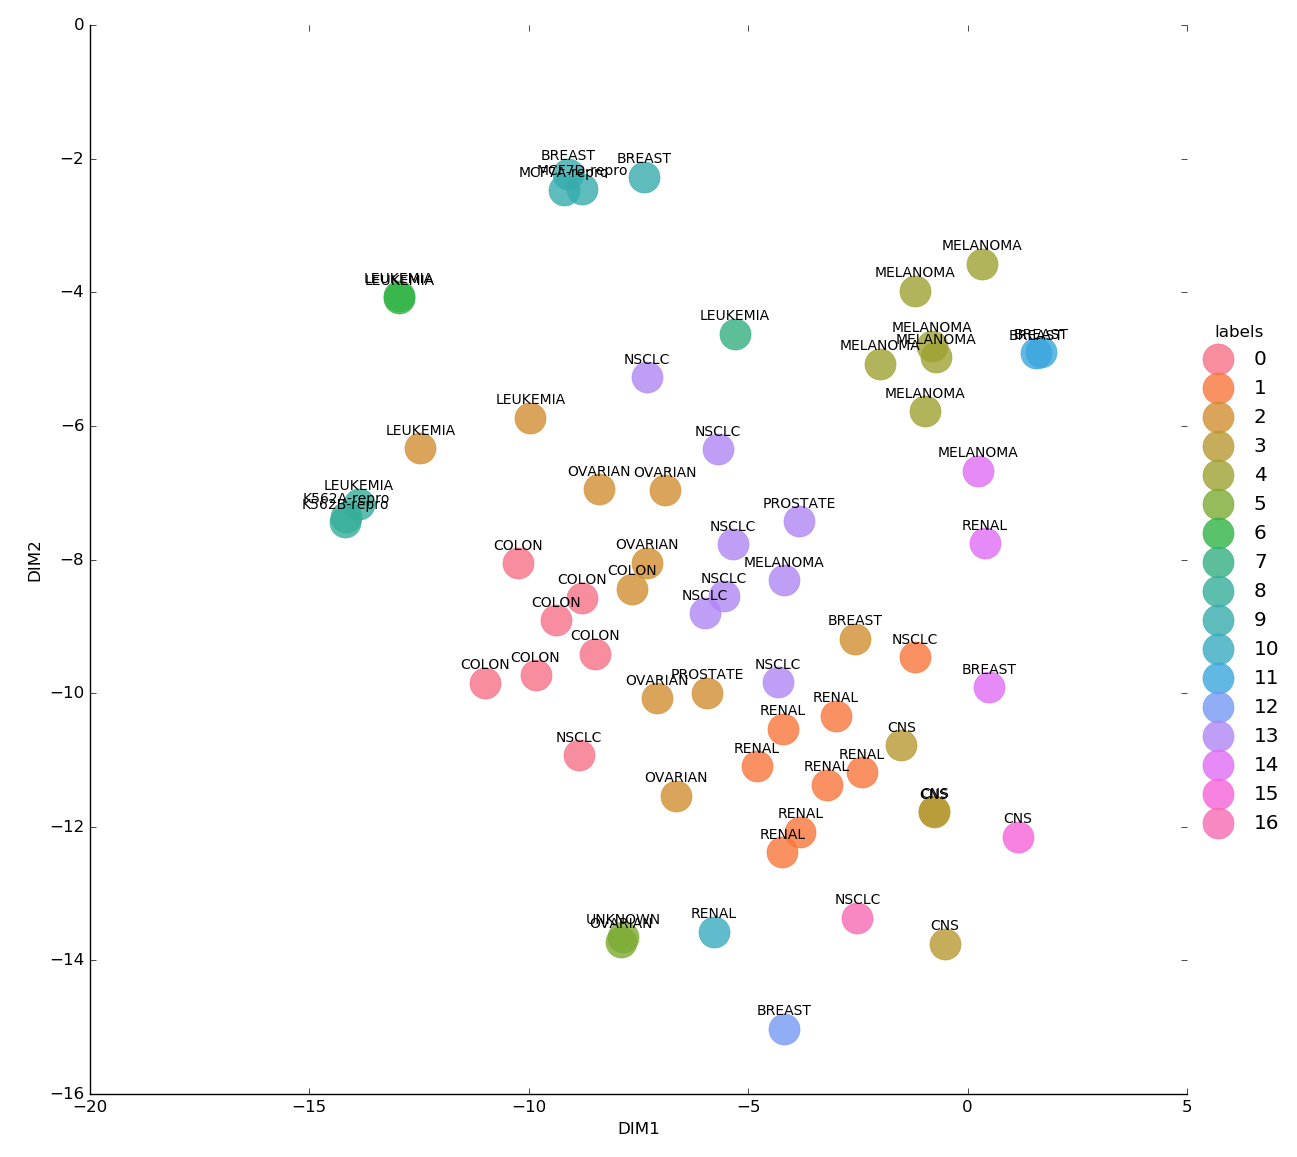
\includegraphics[width=\linewidth]{./figures/best_clustering_labels1.png}
   	\end{subfigure}
\end{figure}
\newpage

And the print of the actual cluster groupings:
\begin{verbatim}
0  | ['COLON', 'COLON', 'COLON', 'COLON', 'COLON', 'COLON', 'NSCLC']
1  | ['RENAL', 'RENAL', 'RENAL', 'RENAL', 'RENAL', 'RENAL', 'RENAL', 'NSCLC']
2  | ['BREAST', 'OVARIAN', 'OVARIAN', 'OVARIAN', 'OVARIAN', 'OVARIAN', 
      'PROSTATE', 'LEUKEMIA', 'LEUKEMIA', 'COLON']
3  | ['CNS', 'CNS', 'CNS', 'CNS']
4  | ['MELANOMA', 'MELANOMA', 'MELANOMA', 'MELANOMA', 'MELANOMA', 'MELANOMA']
5  | ['UNKNOWN', 'OVARIAN']
6  | ['LEUKEMIA', 'LEUKEMIA']
7  | ['LEUKEMIA']
8  | ['K562B-repro', 'K562A-repro', 'LEUKEMIA']
9  | ['MCF7A-repro', 'BREAST', 'MCF7D-repro', 'BREAST']
10 | ['RENAL']
11 | ['BREAST', 'BREAST']
12 | ['BREAST']
13 | ['NSCLC', 'MELANOMA', 'PROSTATE', 'NSCLC', 'NSCLC', 'NSCLC', 'NSCLC', 'NSCLC']
14 | ['RENAL', 'BREAST', 'MELANOMA']
15 | ['CNS']
16 | ['NSCLC']
\end{verbatim}
As you can see, we still have one gorup that manages to catch a lot of the data, and is still quite noisy, but it is no longer largely shared by 2 competing groups.  Instead it seems to be filled with a handful of outliers.  We also have a few more groups whom are groups of one.  I'm not sure of the positive or negative significance of this, but the signals from the groups will be clearer.  After some more optimization of t-SNE, we have a plot:

\newpage
\begin{figure}[!htbp]
  	\centering
   	\begin{subfigure}[p]{1.2\linewidth}
    	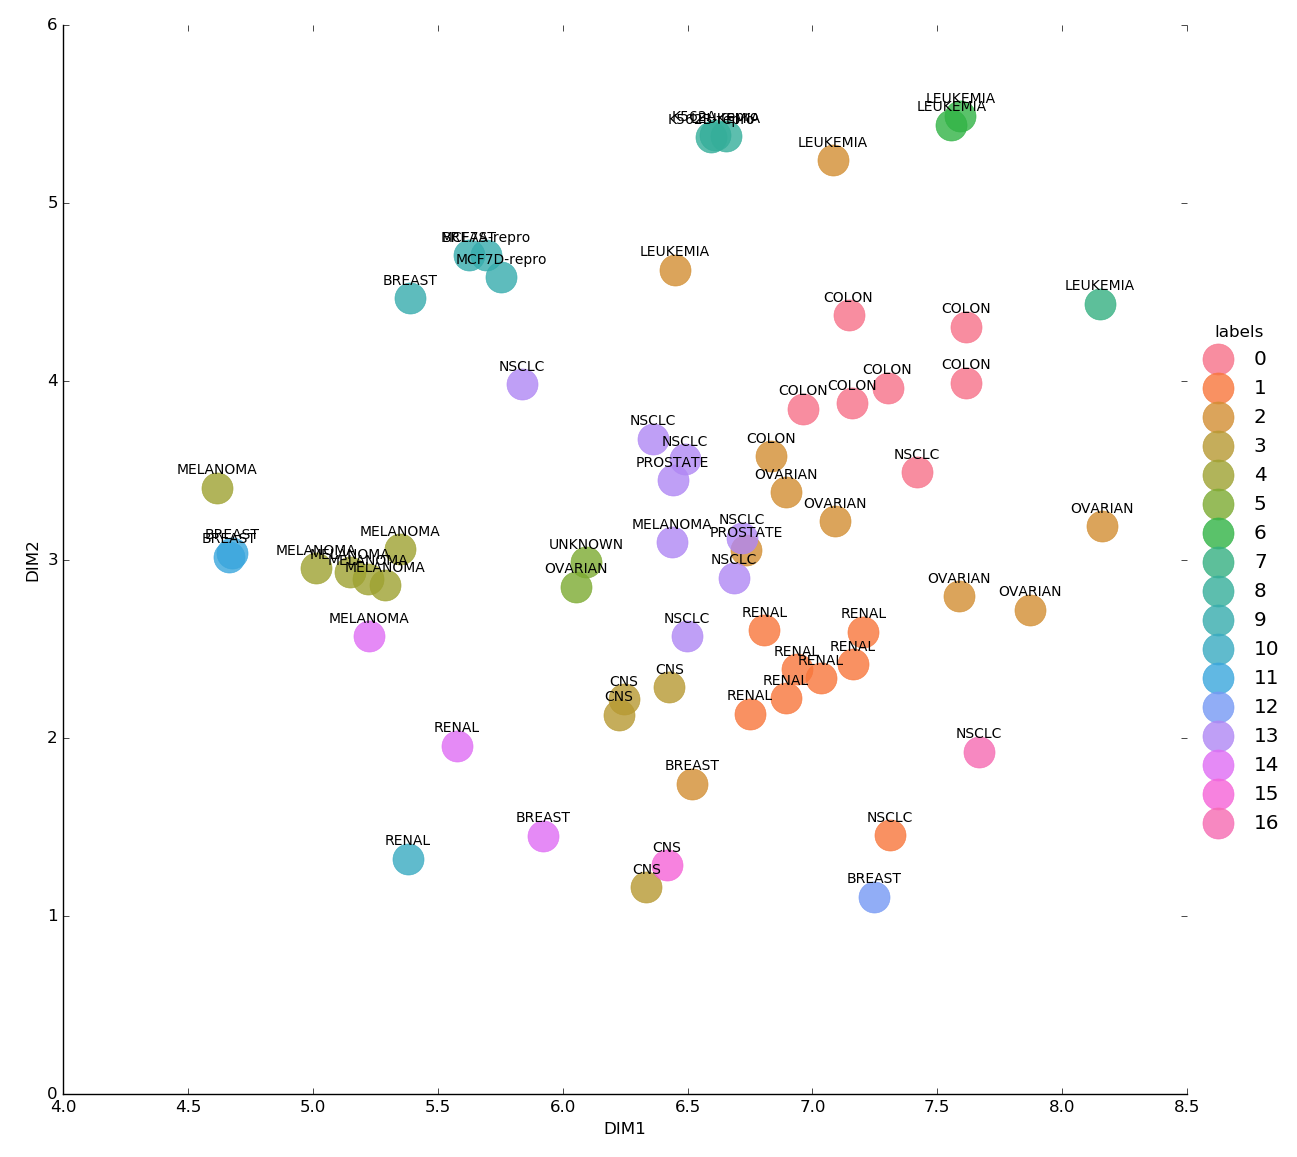
\includegraphics[width=\linewidth]{./figures/another_tsne.png}
   	\end{subfigure}
\end{figure}
Interestingly, even though some labels belong to different clusters (e.g. the \textbf{melanoma} group) the data is still nearby in the output of t-SNE.

\section{Conclusion}
My selection for the algorithms I chose is due to the determinism: That is, I wanted the results to be interpretable.  In addition, many of these clusterings are entirely clean.  If we allow for my defitinition of misclassification, that is, an observation is misclassified if and only if it is in a cluster whose mode does not match the label, then this model has an accuracy of 75\%, using only the natural structuring of the data.  However, we were able to tune model by selecting hyper-parameters which minimized my mis-classification metric.  If we were given no labels at all, then those initial results proposed in the beginning of the paper look completely sufficient, and it would require help from the studying body (The group of people who provided the dataset to us) to verify the results of that clustering.

\section{References}
\begin{enumerate}
\item Wattenberg, et al., "How to Use t-SNE Effectively", Distill, 2016. \url{http://doi.org/10.23915/distill.00002}
\item Keitakurita, "Paper Dissected: 'Visualizing Data using t-SNE' Explained", mlexplained.com, 2018. \url{http://mlexplained.com/2018/09/14/paper-dissected-visualizing-data-using-t-sne-explained/}
\end{enumerate}

\end{document}






































